\documentclass[12pt,spanish,a5paper,landscape]{article}
\usepackage[utf8]{inputenc}
\usepackage{babel}
\usepackage{listings}
\usepackage{mathpazo}
\usepackage{courier}
\usepackage{xcolor}
\usepackage{textcomp}
\usepackage{amsmath}
\usepackage{amssymb}
\usepackage{tikz}
\usepackage{geometry}
\usepackage{enumitem}

\newcommand{\onelinerule}{\rule[2.3ex]{0pt}{0pt}}
\newcommand{\twolinerule}{\rule[6.2ex]{0pt}{0pt}}
\newcommand{\respuesta}{\framebox[\textwidth]{\twolinerule}}
\newcommand{\nombre}{%
  \begin{tikzpicture}[xscale=.4,yscale=.7]
    \draw (0, 0) rectangle (22, 1);
  \end{tikzpicture}%
}
%\newcommand{\rol}   {\framebox[0.3\textwidth]{\onelinerule}}
\newcommand{\rol}{%
  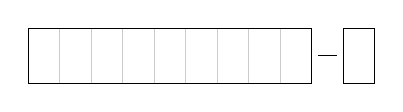
\begin{tikzpicture}[xscale=.4,yscale=.7]
    \draw[gray!40] ( 0, 0) grid      ( 9, 1);
    \draw          ( 0, 0) rectangle ( 9, 1);
    \draw          (10, 0) rectangle (11, 1);
    \draw (9 + .2, .5) -- (10 - .2, .5);
  \end{tikzpicture}%
}
\newcommand{\li}{\lstinline}
\newcommand{\pond}[1]{[{\small\textbf{#1\%}}]}

\lstdefinelanguage{py}{%
  classoffset=0,%
    morekeywords={%
      False,class,finally,is,return,None,continue,for,lambda,try,%
      True,def,from,nonlocal,while,and,del,global,not,with,print,%
      as,elif,if,or,yield,assert,else,import,pass,break,except,in,raise},%
    keywordstyle=\color{black!80}\bfseries,%
  classoffset=1,
    morekeywords={int,float,str,abs,len,raw_input,exit,range,min,max,%
      set,dict,tuple,list,bool,complex,round,sum,all,any,zip,map,filter,%
      sorted,reversed,dir,file,frozenset,open,%
      array,zeros,ones,arange,linspace,eye,diag,dot},
    keywordstyle=\color{black!50}\bfseries,%
  classoffset=0,%
  sensitive=true,%
  morecomment=[l]\#,%
  morestring=[b]',%
  morestring=[b]",%
  stringstyle=\em,%
}

\lstdefinelanguage{testcase}{%
  moredelim=[is][\bfseries]{`}{`},%
  backgroundcolor=\color{gray!20},%
}

\lstdefinelanguage{file}{%
  frame=single,%
  backgroundcolor=\color{white},%
}

\lstset{language=py}
\lstset{basicstyle=\ttfamily}
\lstset{columns=fixed}
\lstset{upquote=true}
\lstset{showstringspaces=false}
\lstset{rangeprefix=\#\ }
\lstset{includerangemarker=false}

\newlist{certamen}{enumerate}{1}
\setlist[certamen]{%
  label=\arabic*.,
  font=\LARGE\bfseries,%
  labelindent=-.5in,%
  leftmargin=0pt,%
  labelsep=1em%
}


\lstset{frame=single}
\lstset{language=testcase}

\parskip 1ex
\parindent 0pt

\newcommand\nc{2}

\begin{document}
  \pagestyle{empty}
  \thispagestyle{empty}

  \part*{Control \nc, lunes 1--2}
  \newpage

  La Progratón 2012 espera recaudar veinte mil pesos.
  Apenas se logre la meta,
  se dejará de aceptar donaciones.

  Escriba un programa que reciba todas las donaciones.
  Al final,
  el programa debe agradecer
  al donante que más aportó.
  En caso de que sean varios,
  sólo hay que agradecer al primero.

  \lstinputlisting{casos-lunes-1-2.txt}

  \newpage
  \part*{Control \nc, lunes 3--4}
  \newpage

  Para pagar su deuda de doscientos mil pesos,
  Prisciliano venderá artículos de su colección personal.

  La colección incluye
  estampillas de 30 mil pesos,
  jarrones de 80 mil pesos y
  sombreros de 40 mil pesos.

  Escriba un programa
  que reciba los artículos que serán vendidos
  hasta que la deuda haya sido saldada.
  Además,
  el programa debe mostrar
  cuántas unidades de cada artículo
  fueron vendidas.

  \lstinputlisting{casos-lunes-3-4.txt}

  \newpage
  \part*{Control \nc, martes 1--2}
  \newpage

  Un vendedor sale de Santiago
  para hacer varios viajes.
  Los viajes hacia el norte
  se representan con kilometrajes positivos,
  y hacia el sur con kilometrajes negativos.

  Escriba un programa que pida al vendedor
  ingresar los kilometrajes de sus via\-jes
  hasta que regrese a su lugar de partida.
  Al final,
  el programa debe mostrar
  la distancia total recorrida
  y la cantidad de viajes hechos
  hacia el norte y hacia el sur.

  \lstinputlisting{casos-martes-1-2.txt}

  \newpage
  \part*{Control \nc, martes 3--4}
  \newpage

  La asignatura de Programología
  tiene varios certámenes,
  evaluados con nota de 0 a 100.
  La profesora decidió eliminar
  la peor y la mejor nota de cada alumno
  antes de calcular el promedio final.

  Escriba un programa que pregunte
  las notas de un alumno,
  y le muestre su nota final.
  El programa debe preguntar al principio
  cuántas notas serán ingresadas.

  \lstinputlisting{casos-martes-3-4.txt}


\end{document}

